\documentclass[12pt, letterpaper]{article}

\usepackage[utf8]{inputenc}
\usepackage{float}
\usepackage{systeme}
\usepackage{amsmath}
\usepackage{amssymb}
\usepackage{enumitem}
\usepackage{amsfonts}
\usepackage{amsthm}
\usepackage{graphicx}
\usepackage[colorinlistoftodos]{todonotes}
\usepackage{pifont}
\usepackage{mdframed,color}
\usepackage[letterpaper, left=3cm, right=3cm, top=3cm, bottom=3cm]{geometry}
\newcommand{\Z}{\mathbb{Z}}
\newcommand{\N}{\mathbb{N}}
\newcommand{\C}{\mathbb{C}}
\newcommand{\Q}{\mathbb{Q}}
\newcommand{\R}{\mathbb{R}}
\newcommand{\F}{\mathbb{F}}
\newtheoremstyle{statement}{3pt}{3pt}{}{}{\bfseries}{:}{.5em}{}

\theoremstyle{statement}
\newtheorem*{atmProp}{Proposition}

\theoremstyle{statement}
\newtheorem*{atmStat}{Statement}

\newenvironment{atmProof}{\noindent\ignorespaces\paragraph{Proof:}}{\hfill \ding{122}\par\noindent}

\newenvironment{Solution}{\noindent\ignorespaces\paragraph{Solution:}}{\hfill \ding{122}\par\noindent}

\newcount\arrowcount
\newcommand\arrows[1]{
        \global\arrowcount#1
        \ifnum\arrowcount>0
                \begin{matrix}
                \expandafter\nextarrow
        \fi
}

\newcommand\nextarrow[1]{
        \global\advance\arrowcount-1
        \ifx\relax#1\relax\else \xrightarrow{#1}\fi
        \ifnum\arrowcount=0
                \end{matrix}
        \else
                \\
                \expandafter\nextarrow
        \fi
}

\title{1.9/2.1 Extra Credit Question}
\author{Rafael Laya}
\date{Fall 2018}

\begin{document}
    \maketitle

    \begin{atmStat}
    A rectangle has vertices $O(0, 0, 0), A(5, 0, 0), B(5, 3, 0),$ and $C(0, 3, 0)$ in the xy plane. A linear transformation $\operatorname{T}$ takes the vertices of the rectangle $OABC$ to $O'(0, 0, 0), A'(0, 3, 4), B'(3, 3, 4),$ and $C'(3, 0, 0)$
    \end{atmStat}
    a) Find matrices that represent successive rigid rotations of space that will describe this transformation. (This can be done in two or three steps).
    
    b) Check that the vertices of $OABC$ are actually transformed to the vertices of $O$’$A$’$B$’$C$’.
    
    c) This transformation can be described as a rotation about a single axis.  Find that axis of rotation.

    \begin{Solution}
    a)
    We begin by making a plot of the rectangle $OABC$ and $O$'$A$'$B$'$C$
    
    \begin{figure}[H]
        \centering
        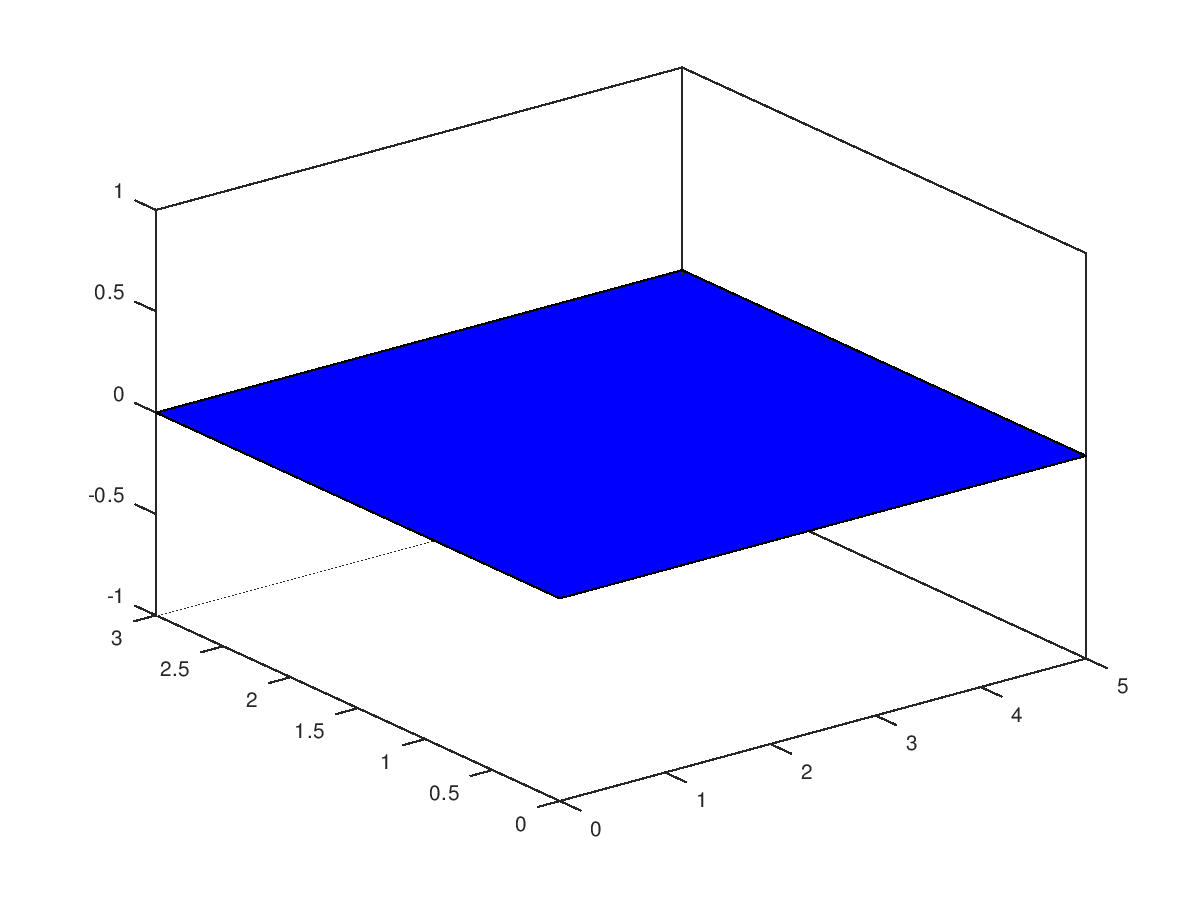
\includegraphics[scale=0.5]{box1.png}
        \caption{The Rectangle OABC}
        \label{fig:fig1}
    \end{figure}
    
    \begin{figure}[H]
        \centering
        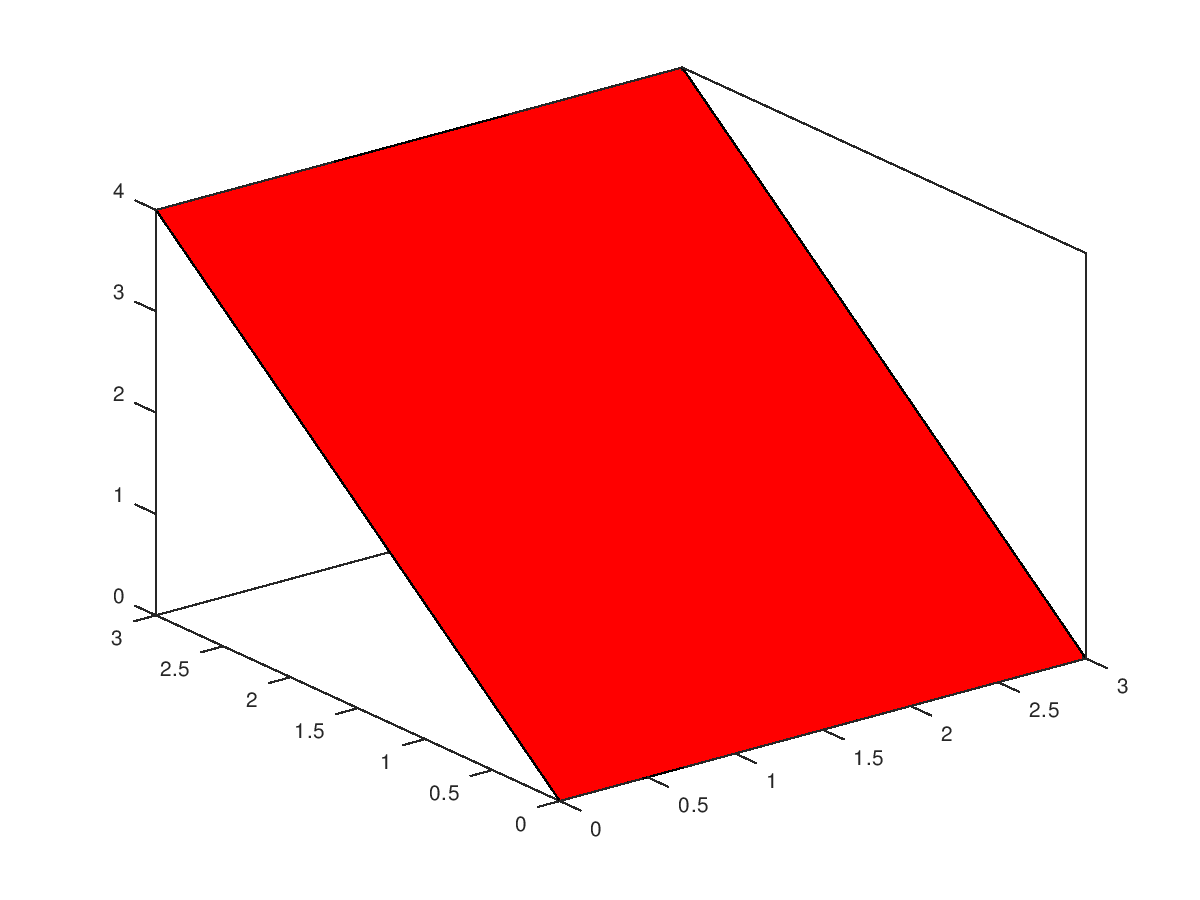
\includegraphics[scale=0.5]{box2.png}
        \caption{The Rectangle $O$'$A$'$B$'$C$'}
        \label{fig:fig2}
    \end{figure}
    
    \begin{figure}[H]
        \centering
        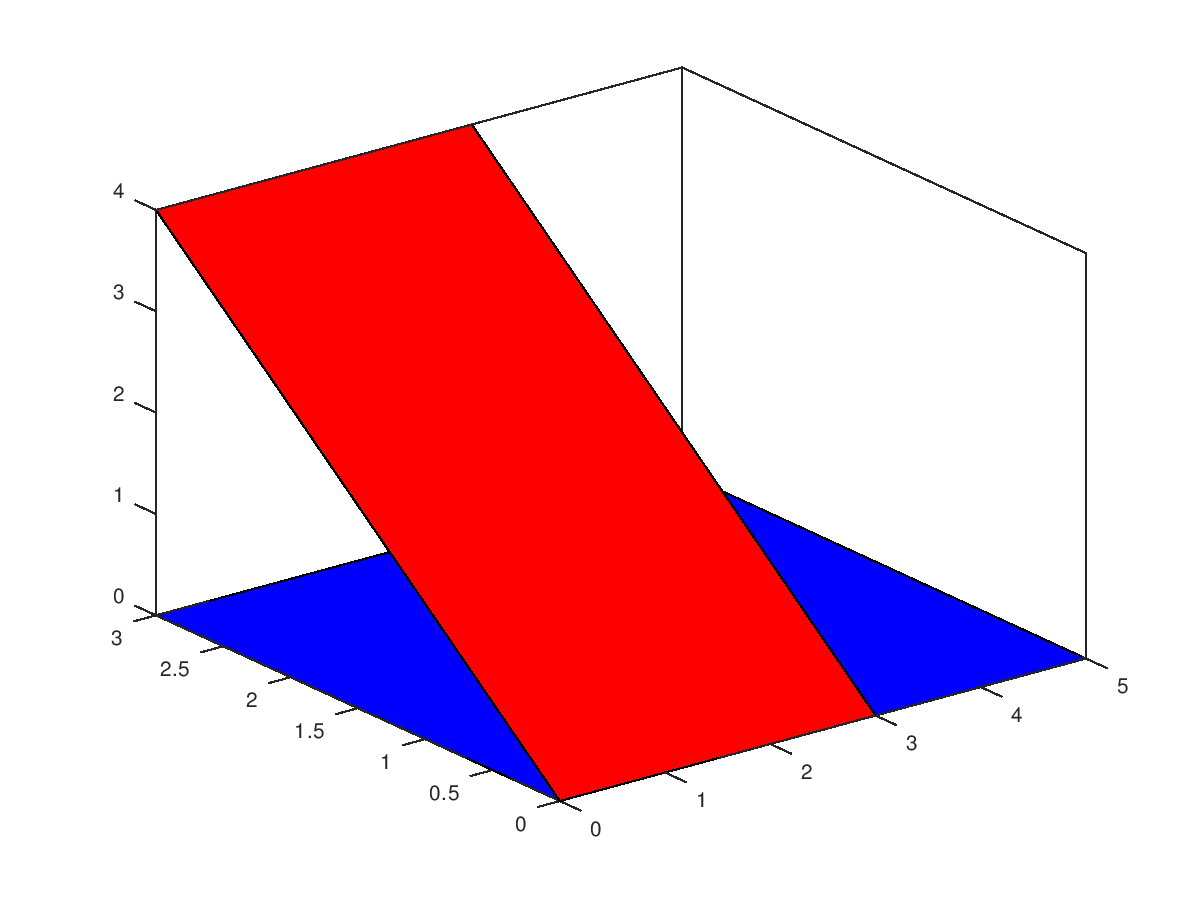
\includegraphics[scale=0.5]{box3.png}
        \caption{Both Rectangles}
        \label{fig:fig3}
    \end{figure}
    
    For ease of writing I am going to call a rotation about an axis $x, y$ or $z$ with angle $\theta$ to the counterclockwise rotation about any of these three axis when the axis is pointing to the observer (This is the direction in which the other four fingers point when the thumb is positioned in the axis when using the right-hand rule). My goal is to rotate the blue rectangle $-\frac{\pi}{2}$ about the $z$ axis. After that we will need another rotation of $-\frac{\pi}{2}-\beta$ ($\beta$ is an unknown angle which we will worry about later) about the $x$ axis. This will describe the transformation and I will provide pictures after I have made a successful rotation. I will show that the transformation does indeed what the images show in part (b).
    
    \subsection*{Rotation of $-\frac{\pi}{2}$ about the $z$ axis}
    
    We showed in class that the rotation matrix about the $z$ axis of angle $\theta$ is:
    
    $$
    A_1=
    \begin{bmatrix}
    \cos{\theta} & -\sin{\theta} & 0 \\
    \sin{\theta} & \cos{\theta} & 0 \\
    0 & 0 & 1
    \end{bmatrix}
    $$
    
    When $\theta=-\frac{\pi}{2}$ We have the matrix that represents the transformation $\operatorname{T_1}:\R^3\longrightarrow\R^3$ such that $\operatorname{T_1}(\Vec{x})=A_1\Vec{x}$:
    
    $$
    A_1=
    \begin{bmatrix}
    0 & 1 & 0 \\
    -1 & 0 & 0 \\
    0 & 0 & 1
    \end{bmatrix}
    $$
    
    \begin{figure}[H]
        \centering
        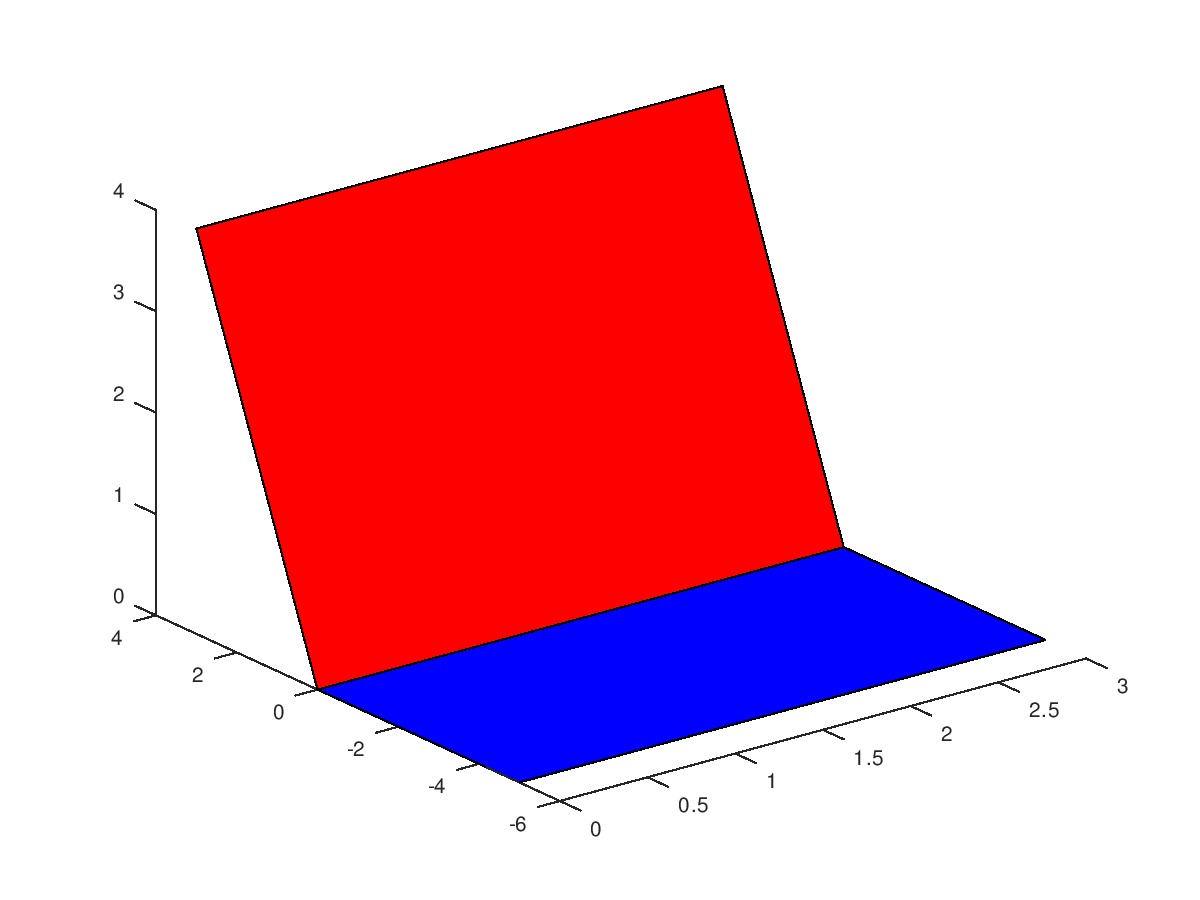
\includegraphics[scale=0.5]{box4.png}
        \caption{The blue rectangle has undergone its first rotation}
        \label{fig:fig4}
    \end{figure}
    
    \end{Solution}
    
    \subsection*{Rotation of $-\frac{\pi}{2}-\beta$ about the $x$ axis}
    In class we showed the rotation matrix about the $x$ axis with angle $\theta$ is given by:
    
    $$
    A_2=
    \begin{bmatrix}
    1 & 0 & 0\\
    0 & \cos{\theta} & -\sin{\theta} \\
    0 & \sin{\theta} & \cos{\theta}  
    \end{bmatrix}
    $$
    
    Let $\theta=-\frac{\pi}{2}-\beta$
    $$
    A_2=
    \begin{bmatrix}
    1 & 0 & 0\\
    0 & \cos({-\frac{\pi}{2}-\beta}) & -\sin({-\frac{\pi}{2}-\beta}) \\
    0 & \sin({-\frac{\pi}{2}-\beta}) & \cos({-\frac{\pi}{2}-\beta})  
    \end{bmatrix}
    $$
    
    Recall that $\cos(x)$ is an even function while $\sin(x)$ is an odd function,
    
    $$
    A_2=
    \begin{bmatrix}
    1 & 0 & 0\\
    0 & \cos({\frac{\pi}{2}+\beta}) & \sin({\frac{\pi}{2}+\beta}) \\
    0 & -\sin({\frac{\pi}{2}+\beta}) & \cos({\frac{\pi}{2}+\beta})
    \end{bmatrix}
    $$
    Also, $cos(x+\frac{\pi}{2})$=$-sin(x)$ and $sin(x+\frac{\pi}{2})=cos(x)$, therefore:
    
    $$
    A_2=
    \begin{bmatrix}
    1 & 0 & 0\\
    0 & -\sin(\beta) & \cos(\beta) \\
    0 & -\cos(\beta) & -\sin(\beta) 
    \end{bmatrix}
    $$
    
    We have to figure out the values $cos(\beta), sin(\beta)$. By projecting the red rectangle on the $yz$ plane, $\beta$ is the angle between the vertical ($z$) axis and the red line (which corresponds to the projection of the red rectangle):
    
    \begin{figure}[H]
        \centering
        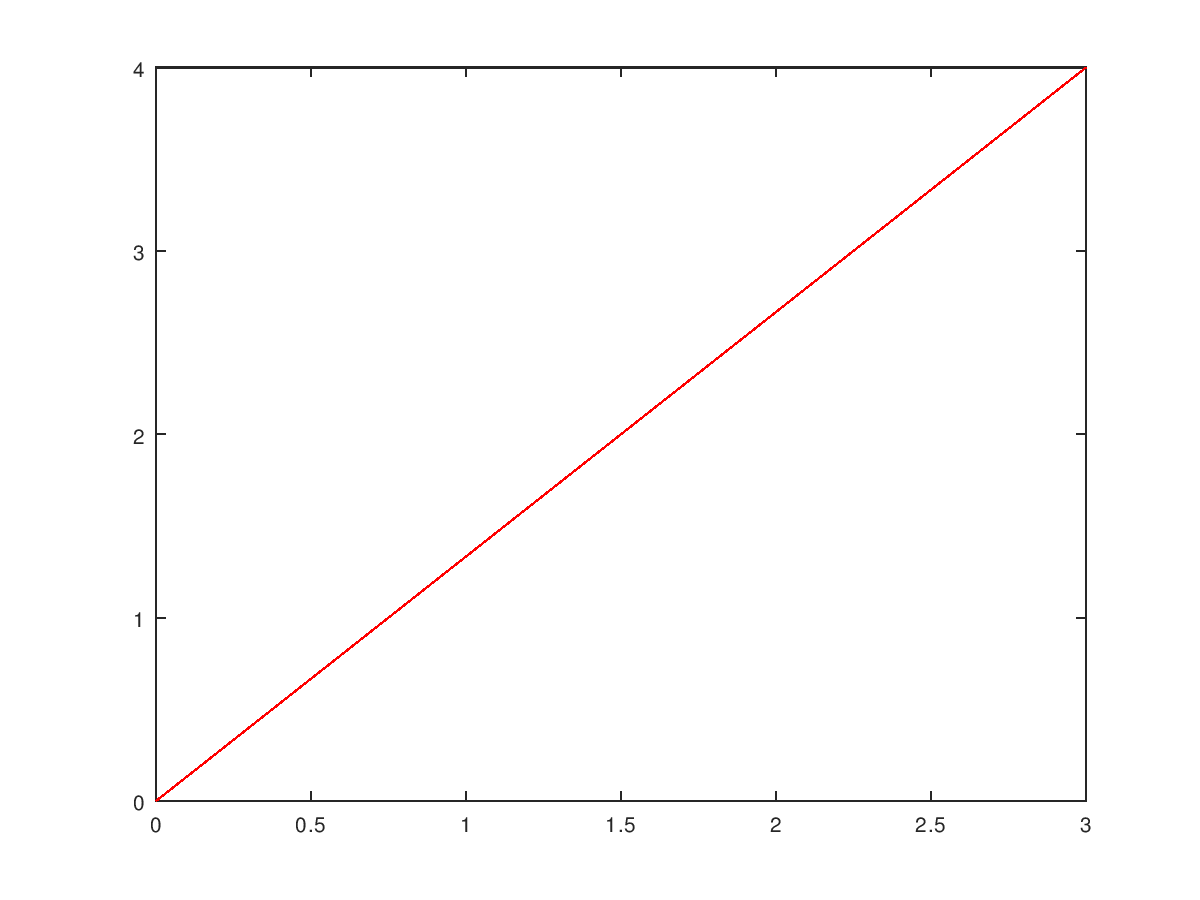
\includegraphics[scale=0.5]{line1.png}
        \caption{The Projection on the plane yz of the target rectangle}
        \label{fig:line1}
    \end{figure}
    
    Using Pythagora's Theorem the hypothenuse measures $\sqrt{4^2+3^2}=\sqrt{16+9}=\sqrt{25}=5$ and therefore $sin(\beta) = \frac{3}{5}$ and $cos(\beta) = \frac{4}{5}$. Finally, the matrix $A_2$ that represents the rotation we wanted by the linear transformation $\operatorname{T_2}:\R^3\longrightarrow\R^3$ such that $\operatorname{T_2}(\Vec{x})=A_2\Vec{x}$ is:
    
    $$
    A_2=
    \begin{bmatrix}
    1 & 0 & 0\\
    0 & -\frac{3}{5}& \frac{4}{5} \\
    0 & -\frac{4}{5} & -\frac{3}{5} 
    \end{bmatrix}
    $$
    
    \begin{figure}[H]
        \centering
        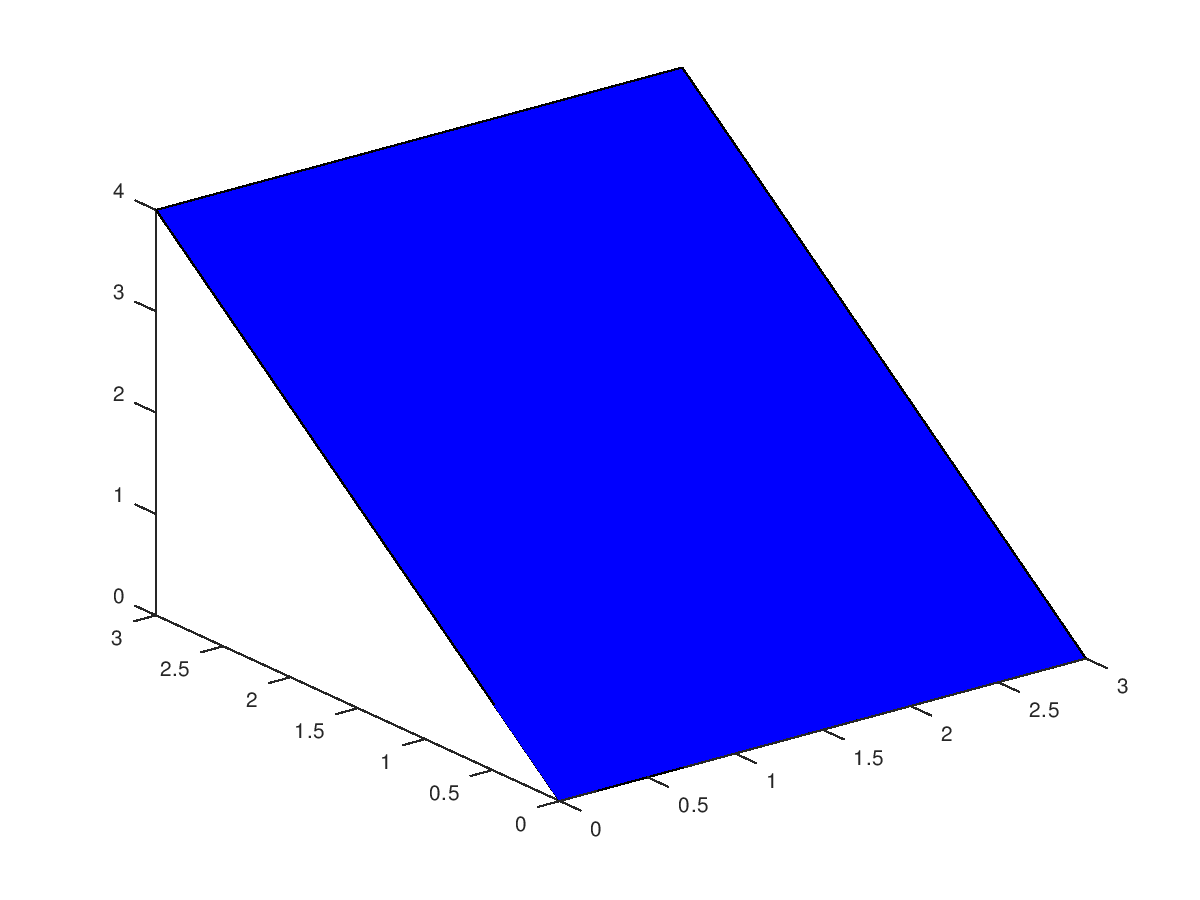
\includegraphics[scale=0.5]{boxfin.png}
        \caption{The blue rectangle after the two transformations $T_1$ and then $T_2$}
        \label{fig:finalTransformed}
    \end{figure}
    
    b) Let $\Vec{x}=\begin{bmatrix} x_1 \\ x_2 \\ x_3\end{bmatrix}\in\R^3$. The net transformation is: $\operatorname{T}:\R^3\longrightarrow\R^3$ is $\operatorname{T}(\Vec{x})=A_2(A_1\Vec{x})=(A_2A_1)\Vec{x}$. Let's multiply $A_2A_1$ (Properties of matrix multiplication allow for this):
    
    $$
    A_2A_1 = 
    \begin{bmatrix}
    1 & 0 & 0\\
    0 & -\frac{3}{5}& \frac{4}{5} \\
    0 & -\frac{4}{5} & -\frac{3}{5} 
    \end{bmatrix}
    \begin{bmatrix}
    0 & 1 & 0 \\
    -1 & 0 & 0 \\
    0 & 0 & 1
    \end{bmatrix}
    =
    \begin{bmatrix}
    0 & 1 & 0 \\
    \frac{3}{5} & 0 & \frac{4}{5} \\
    \frac{4}{5} & 0 & -\frac{3}{5}
    \end{bmatrix}
    $$
    And as such:
    $$
    \operatorname{T}(\Vec{x})
    =
    \begin{bmatrix}
    0 & 1 & 0 \\
    \frac{3}{5} & 0 & \frac{4}{5} \\
    \frac{4}{5} & 0 & -\frac{3}{5}
    \end{bmatrix}
    \Vec{x}
    =
    \begin{bmatrix}
    0 & 1 & 0 \\
    \frac{3}{5} & 0 & \frac{4}{5} \\
    \frac{4}{5} & 0 & -\frac{3}{5}
    \end{bmatrix}
    \begin{bmatrix}
    x_1 \\ x_2 \\ x_3
    \end{bmatrix}
    =
    \begin{bmatrix}
    x_2 \\
    \frac{3x_1+4x_3}{5} \\
    \frac{4x_1-3x_3}{5}
    \end{bmatrix}
    $$
    Let's now check that our transformation does transform the vertices $OABC$ to $O$'$A$'$B$'$C$'. We can represent these vertices as vectors that point to each vertex by simply using the coordinates of the point in the same order as entries in the vector, for instance $\Vec{A}=\begin{bmatrix} 5 \\0\\0\end{bmatrix}$ corresponds to the vertex $A$. 
    
    $$
    \operatorname{T}(\Vec{A})
    =\operatorname{T}\left(\begin{bmatrix}
                        5\\ 0\\ 0
                        \end{bmatrix}\right)
    =\begin{bmatrix}
    0\\
    \frac{3(5)+4(0)}{5}\\
    \frac{4(5)-3(0)}{5}
    \end{bmatrix}
    =\begin{bmatrix}
    0\\
    3\\
    4
    \end{bmatrix}
    =\Vec{A'}
    $$
    
    $$
    \operatorname{T}(\Vec{B})
    =\operatorname{T}\left(\begin{bmatrix}
                        5 \\3 \\0
                        \end{bmatrix}\right)
    =\begin{bmatrix}
    3\\
    \frac{3(5)+4(0)}{5}\\
    \frac{4(5)-3(0)}{5}
    \end{bmatrix}
    =\begin{bmatrix}
    3\\
    3\\
    4
    \end{bmatrix}
    =\Vec{B'}
    $$
    
    $$
    \operatorname{T}(\Vec{C})
    =\operatorname{T}\left(\begin{bmatrix}
                        0\\ 3 \\0
                        \end{bmatrix}\right)
    =\begin{bmatrix}
    3\\
    \frac{3(0)+4(0)}{5}\\
    \frac{4(0)-3(0)}{5}
    \end{bmatrix}
    =\begin{bmatrix}
    3\\
    0\\
    0
    \end{bmatrix}
    =\Vec{C'}
    $$
    
    $$
    \operatorname{T}(\Vec{O})
    =\operatorname{T}\left(\begin{bmatrix}
                        0 \\0 \\0
                        \end{bmatrix}\right)
    =\begin{bmatrix}
    0\\
    \frac{3(0)+4(0)}{5}\\
    \frac{4(0)-3(0)}{5}
    \end{bmatrix}
    =\begin{bmatrix}
    0\\
    0\\
    0
    \end{bmatrix}
    =\Vec{O'}
    $$
    
    c) When a rotation occurs about some axis that goes through the origin then any vector in the axis of the rotation gets mapped into itself (and because these transformations are linear the origin is always mapped to the origin and therefore only rotations about an axis that goes through the origin are allowed, because if the axis does not go through the origin then the origin will move with the rotation). That is, if $L$ is the axis of rotation take some $\Vec{x}\in\R^3$ such that $\Vec{x}\in L$ and apply some rotation $\operatorname{T}$, then $\operatorname{T}(\Vec{x})=\Vec{x}$. That is,
    
    $$
    \operatorname{T}(\Vec{x})
    =\operatorname{T}\left(\begin{bmatrix} x_1\\x_2\\x_3\end{bmatrix}\right)
    =
    \begin{bmatrix}
    x_2 \\
    \frac{3x_1+4x_3}{5}\\
    \frac{4x_1-3x_3}{5}
    \end{bmatrix}
    =\begin{bmatrix}
    x_1\\x_2\\x_3
    \end{bmatrix}
    $$
    
    Then,
    
    \systeme{x_2=x_1, \frac{3}{5}x_1+\frac{4}{5}x_3=x_2,
    \frac{4}{5}x_1-\frac{3}{5}x_3=x_3}\\
    
    
    or\\
    
    
    \systeme{-x_1+x_2=0, 3x_1-5x_2+4x_3=0, 4x_1-8x_3=0}
    
    Row Reducing the Augmented Matrix associated to the System above, 
    
    $$
    \begin{bmatrix}
    -1 & 1 & 0 & 0 \\
    3 & -5 & 4 & 0 \\
    4 & 0 & -8 & 0
    \end{bmatrix}
    \arrows3{-R_1}{}{}
    \begin{bmatrix}
    1 & -1 & 0 & 0 \\
    3 & -5 & 4 & 0 \\
    4 & 0 & -8 & 0
    \end{bmatrix}
    \arrows3{}{R_2-3R_1}{R_3-4R_1}
    \begin{bmatrix}
    1 & -1 & 0 & 0 \\
    0 & -2 & 4 & 0 \\
    0 & 4 & -8 & 0
    \end{bmatrix}
    \arrows3{}{\frac{-1}{2}R_2}{}
    \begin{bmatrix}
    1 & -1 & 0 & 0 \\
    0 & 1 & -2 & 0 \\
    0 & 4 & -8 & 0
    \end{bmatrix}
    $$
    $$
    \arrows3{R_1+R_2}{}{R_3-4R_2}
    \begin{bmatrix}
    1 & 0 & -2 & 0 \\
    0 & 1 & -2 & 0 \\
    0 & 0 & -0 & 0
    \end{bmatrix}
    $$
    
    Thus the solution to the system is:
    
    \systeme{x_1-2x_3=0, x_2-2x_3=0}; $x_3$ is free\\
    
    In Parametric form.\\
    
    \systeme{x_1=2t, x_2=2t, x_3=t}\\
    
    Which is the equation of a line through $\begin{bmatrix} 0 \\ 0 \\ 0\end{bmatrix}$ and in the direction of $\begin{bmatrix} 2\\2\\1\end{bmatrix}$. The axis of rotation is the line $L$:\\
    
    $L:$ \systeme{x_1=2t,x_2=2t,x_3=t}
    
\end{document}
